\chapter{Исследовательская часть}

В данном разделе лабораторной работы будут приведены примеры работы программы, а также выполнена сравнительная характеристика алгоритма с распараллеливанием и без.

\section{Технические характеристики устройства}

Ниже представлены характеристики компьютера, на котором проводилось тестирование программы:
\begin{itemize}
    \item операционная система Windows 10 Домашняя 21H2;
    \item оперативная память 16 Гб;
    \item процессор Intel(R) Core(TM) i7-10870H CPU @ 2.20 ГГц.
\end{itemize}

Во время тестирования ноутбук был подключен к сети электропитания. Из программного обеспечения были запущены только среда разработки \textit{PyCharm} и браузер \textit{Chrome}.

Процессор был загружен на 19\%, оперативная память -- на 50\%.

\section{Демонстрация работы программы}

На рисунке \ref{img:example} представлен результат программы по работе алгоритма с распараллеливанием. Выбран 1 пункт меню.

\begin{figure}[h!]
		\center{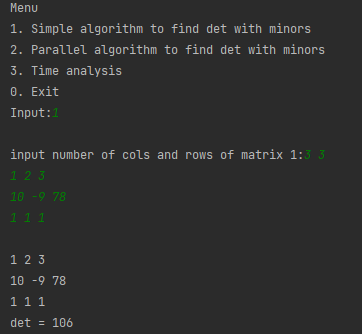
\includegraphics[scale=1]{img/example.png}} % height
		\caption{Пример работы программы}
		\label{img:example}
	\end{figure}
%\img{}{example}{Пример работы программы}

\section{Время выполнения реализаций алгоритмов}

В программе используется библиотека time.h, с помощью которой можно получить время, затраченное процессором на выполнение программы, представленное типом clock\_t, или $-1$, если оно неизвестно. Размерность возвращаемого значения определяется при помощи CLOCKS\_PER\_SEC, константы, которая задаёт количество единиц значения времени в одной секунде.

Использовать функцию приходится дважды, в первый раз перед началом алгоритма, второй — после, а затем из конечного времени необходимо вычесть начальное, чтобы получить потраченное на алгоритм время.

Результаты замеров времени работы реализаций методов умножения на различных входных данных (в с) приведены в таблице \ref{tbl:times}. Замеры для одного и того же алгоритма с одними и теми же входными данными производились 10 раз для получения усредненного результата. Для параллельной реализации алгоритма выбрано количество потоков, равное 4, поскольку именно столько логических ядер имеет процессор ноутбука.

\begin{table}[h]
	\begin{center}
		\begin{threeparttable}
			\captionsetup{justification=raggedright,singlelinecheck=off}
			\caption{\label{tbl:times}Результаты замеров времени}
			\begin{tabular}{|c|c|c|c|}
				\hline
				Размеры сцены &4 потока &без многопоточности\\
				\hline
				1x1 & 0.0006 & 5\\ 
				\hline
				10x10 & 0.001515 & 74\\ 
				\hline
				20x20 & 0.002379 & 141\\ 
				\hline
				30x30 & 0.003276 & 148\\ 
				\hline
				40x40 & 0.004691 & 164\\ 
				\hline
				50x50 & 0.004543 & 184\\
				\hline
			\end{tabular}
		\end{threeparttable}
	\end{center}
\end{table}

Теоретические результаты замеров и полученные практически результаты совпадают.

Также на рисунках \ref{img:graph1} и \ref{img:graph2} приведены графические результаты замеров работы алгоритмы на квадратных матрицах в зависимости от их размера и количества потоков. Введены следующие обозначения: \textit{nm} --- реализация алгоритма без многопоточности, \textit{m4} --- реализация алгоритма с распараллеливанием на 4 потока, \textit{m} --- реализация алгоритма с распараллеливанием на различное количество потоков.
\FloatBarrier
\imgScale{1}{graph1}{Сравнение времени работы алгоритма с распараллеливанием на различное количество потоков при работе с матрицами размером 500x500}
\FloatBarrier
\FloatBarrier
\imgScale{1}{graph2}{Сравнение времени работы алгоритма без распараллеливания и с 4 вспомогательными потоками при работе с квадратными матрицами}
\FloatBarrier

\section*{Вывод}
По графикам видно, что при испольозвании 4 вспомогательных потоков, многопоточная реализация алгоритма  значительно эффективнее по времени реализации без многопоточности при работе с матрицами размером 500x500. Данное количество потоков обусловлено тем, что на ноутбуке, на котором проводились замеры времени ПО, имеется всего 4 логических ядра, а следовательно, количество потоков, при котором потоки будут распределены между всеми ядрами равномерно, равно 4. Именно поэтому лучшие результаты достигаются именно на 4 потоках, даже несмотря на ресурсы, которые дополнительно затрачиваются на содержание потоков. Исходя из построенных графиков, можно сделать вывод, что распараллеливание кода значительно увеличивает эффективность алгоритма поиска определителя матрицы по времени.